%% For double-blind review submission, w/o CCS and ACM Reference (max submission space)
\documentclass[sigplan,review=false,anonymous=false]{acmart}\settopmatter{printfolios=true,printccs=false,printacmref=false}
%% For double-blind review submission, w/ CCS and ACM Reference
%\documentclass[sigplan,review,anonymous]{acmart}\settopmatter{printfolios=true}
%% For single-blind review submission, w/o CCS and ACM Reference (max submission space)
%\documentclass[sigplan,review]{acmart}\settopmatter{printfolios=true,printccs=false,printacmref=false}
%% For single-blind review submission, w/ CCS and ACM Reference
%\documentclass[sigplan,review]{acmart}\settopmatter{printfolios=true}
%% For final camera-ready submission, w/ required CCS and ACM Reference
%\documentclass[sigplan]{acmart}\settopmatter{}


%% Conference information
%% Supplied to authors by publisher for camera-ready submission;
%% use defaults for review submission.

\acmConference[]{}
\acmYear{}
\acmISBN{} % \acmISBN{978-x-xxxx-xxxx-x/YY/MM}
\acmDOI{} % \acmDOI{10.1145/nnnnnnn.nnnnnnn}
\startPage{}

%% Copyright information
%% Supplied to authors (based on authors' rights management selection;
%% see authors.acm.org) by publisher for camera-ready submission;
%% use 'none' for review submission.
\setcopyright{none}
%\setcopyright{acmcopyright}
%\setcopyright{acmlicensed}
%\setcopyright{rightsretained}
\copyrightyear{}           %% If different from \acmYear

%% Bibliography style
\bibliographystyle{ACM-Reference-Format}
%% Citation style
%\citestyle{acmauthoryear}  %% For author/year citations
%\citestyle{acmnumeric}     %% For numeric citations
%\setcitestyle{nosort}      %% With 'acmnumeric', to disable automatic
                            %% sorting of references within a single citation;
                            %% e.g., \cite{Smith99,Carpenter05,Baker12}
                            %% rendered as [14,5,2] rather than [2,5,14].
%\setcitesyle{nocompress}   %% With 'acmnumeric', to disable automatic
                            %% compression of sequential references within a
                            %% single citation;
                            %% e.g., \cite{Baker12,Baker14,Baker16}
                            %% rendered as [2,3,4] rather than [2-4].


%%%%%%%%%%%%%%%%%%%%%%%%%%%%%%%%%%%%%%%%%%%%%%%%%%%%%%%%%%%%%%%%%%%%%%
%% Note: Authors migrating a paper from traditional SIGPLAN
%% proceedings format to PACMPL format must update the
%% '\documentclass' and topmatter commands above; see
%% 'acmart-pacmpl-template.tex'.
%%%%%%%%%%%%%%%%%%%%%%%%%%%%%%%%%%%%%%%%%%%%%%%%%%%%%%%%%%%%%%%%%%%%%%


%% Some recommended packages.
\usepackage{booktabs}   %% For formal tables:
                        %% http://ctan.org/pkg/booktabs
\usepackage{subcaption} %% For complex figures with subfigures/subcaptions
                        %% http://ctan.org/pkg/subcaption
\usepackage{lmodern}
\usepackage{graphicx}
\usepackage{float}
\graphicspath{ {images/} }

\begin{document}

%% Title information
\title{Exploring Floating-Point Trade-Offs in ML}         %% [Short Title] is optional;
                                        %% when present, will be used in
                                        %% header instead of Full Title.
%\titlenote{Both Vanilla and Average variants of the Perceptron algorithm}             %% \titlenote is optional;
                                        %% can be repeated if necessary;
                                        %% contents suppressed with 'anonymous'
%\subtitle{Subtitle}                     %% \subtitle is optional
%\subtitlenote{with sudddddbtitle note}       %% \subtitlenote is optional;
                                        %% can be repeated if necessary;
                                        %% contents suppressed with 'anonymous'


%% Author information
%% Contents and number of authors suppressed with 'anonymous'.
%% Each author should be introduced by \author, followed by
%% \authornote (optional), \orcid (optional), \affiliation, and
%% \email.
%% An author may have multiple affiliations and/or emails; repeat the
%% appropriate command.
%% Many elements are not rendered, but should be provided for metadata
%% extraction tools.

%% Author with single affiliation.
\author{Rocco Salvia}
%\authornote{with author1 note}          %% \authornote is optional;
                                        %% can be repeated if necessary
\orcid{nnnn-nnnn-nnnn-nnnn}             %% \orcid is optional
\affiliation{
  %\position{Position1}
  %\department{Department1}              %% \department is recommended
  \institution{School of Computing - University of Utah}            %% \institution is required
  %\streetaddress{Street1 Address1}
  %\city{City1}
  %\state{State1}
  %\postcode{Post-Code1}
  %\country{Country1}                    %% \country is recommended
}
\email{rocco@cs.utah.edu}          %% \email is recommended

%% Author with two affiliations and emails.
\author{Zvonimir Rakamari\'c}
%\authornote{with author2 note}          %% \authornote is optional;
                                        %% can be repeated if necessary
\orcid{nnnn-nnnn-nnnn-nnnn}             %% \orcid is optional
\affiliation{
  %\position{Position2a}
  %\department{Department2a}             %% \department is recommended
  \institution{School of Computing - University of Utah}           
  %% \institution is required
  %\streetaddress{Street2a Address2a}
  %\city{City2a}
  %\state{State2a}
  %\postcode{Post-Code2a}
  %\country{Country2a}                   %% \country is recommended
}
\email{zvonimir@cs.utah.edu}         %% \email is recommended


%% Abstract
%% Note: \begin{abstract}...\end{abstract} environment must come
%% before \maketitle command
\begin{abstract}
Perceptron and SVM algorithms are two well known linear predictors. Their goal is to build the best hypothesis function given the training data to predict unknown samples in the future. 
Usually, both training and testing procedures are implemented using IEEE 754 double precision, which results in a conservative approach act to minimize the final error of the implementation. 
The main goal of this work is to analyze the impact of floating point precision tuning applied to well known predictors. In particular, we want to determine whether reading the dataset or computing training and testing of the predictor is the most important to the accuracy of the algorithm.
Our analysis spans minimal values of the floating point range, and compare the resulting accuracy to well known IEEE defined standards single and double precision.
\end{abstract}


%% 2012 ACM Computing Classification System (CSS) concepts
%% Generate at 'http://dl.acm.org/ccs/ccs.cfm'.
%\begin{CCSXML}
%<ccs2012>
%<concept>
%<concept_id>10011007.10011006.10011008</concept_id>
%<concept_desc>Software and its engineering~General programming languages</concept_desc>
%<concept_significance>500</concept_significance>
%</concept>
%<concept>
%<concept_id>10003456.10003457.10003521.10003525</concept_id>
%<concept_desc>Social and professional topics~History of programming languages</concept_desc>
%<concept_significance>300</concept_significance>
%</concept>
%</ccs2012>
%\end{CCSXML}

%\ccsdesc[500]{Software and its engineering~General programming languages}
%\ccsdesc[300]{Social and professional topics~History of programming languages}
%% End of generated code
%% Keywords
%% comma separated list
%\keywords{SVM, Perceptron, floating point, consumption.}  %% \keywords are mandatory in final camera-ready submission
%% \maketitle
%% Note: \maketitle command must come after title commands, author
%% commands, abstract environment, Computing Classification System
%% environment and commands, and keywords command.
\maketitle
\section{Introduction}
We use floating point representation because real world characters have to be modeled in the machine. Squeezing infinitely real numbers into a finite number of bits requires an approximate representation\cite{WhatEvery}. 
Developers approach is to be as much conservative as possible about floating point precision: use the maximum precision provided by target platforms\cite{softfloat}. The execution of floating point operations is the major contributor to energy consumption\cite{softfloat}. Approximately 50\% of energy consumption depends on floating point computations\cite{softfloat}.
The impact of low-cost floating point precision on machine learning predictors is an hot topic.\\
Gupta et al.\cite{gupta} prove that deep neural network can be trained using low precision fixed-point arithmetic, with a minimal sacrifice of quality. 
They show how performing fixed point arithmetic using only 16-bit of precision produces same results of IEEE754 single floating point representation (32-bit precision). 

Zhou et al. \cite{dorefa} propose innovative methods to train Convolutional-Neural-Networks (CNNs) with low bit-width weights, activations and gradients. They show how using 1-bit weight, 1-bit activation and 2-bit gradient achieve a value of 93\% of accuracy compared to 97\% obtained with 32-bit single precision. 

Hubara et al.\cite{Hubara} introduce a method to train Quantized-Neural-Networks (QNNs) using low precision arithmetic.
They showed how using 4 bits for weights and activation step result in a degradation of 5.5\% compared to 32-bit single precision.

At the same time, we are aware of many analyzers that are able to scan a black box algorithm to minimize the precision of each floating point instruction while still maintaining the desired value of accuracy. \cite{reducelam}\cite{mixpreclam}\cite{precimonious}\cite{blame}. 

%Program analysis applied to floating point instructions usually maintains few 'ghosts' executions of the program, to replicate the behavior of it with different floating point precisions.\cite{blame}\cite{precimonious}. Once a particular configuration satisfy the evaluation procedure provided by the user, the binary code is altered instructions is injected into the binary code of the program and the candidate result may be evaluated again.\cite{mixpreclam}\cite{reducelam}.

%In particular, the aim of these tools is to produce the minimal configuration of FP instructions such that the output keeps same quality. 
%These techniques involve both static and dynamic approaches: usually the first is used to detect FP instructions in the program, while the second one produces improvement on the configuration of the solution, also due to 'ghost' executions that verify the current configuration.

Our work admire and look forward these analyzers, but we move away from the detection of the minimal floating point configuration of Perceptron and SVM. 

We study what affect the accuracy of these predictors in case of poor floating point precision computations. Our goal is to empirically show how limited can be the floating point format while still maintaining hight accuracy. Also, we report which step in the lifetime of these predictors is most sensitive to precision tuning. 

%We want to compare the accuracy of these predictors ($\frac{Correct.Prediction}{Tot.Samples}$) between minimal values of floating point precision (from 2 to 10 bits for mantissa representation) and well known (and expensive) single and double precisions. %

Our work focuses on tuning the precision of mantissa because we are confident to say that mantissa may show gradual improvement on the final accuracy on the predictor.
On the other hand, the exponent does not exhibit such behavior. 
\begin{figure*}
	\centering
	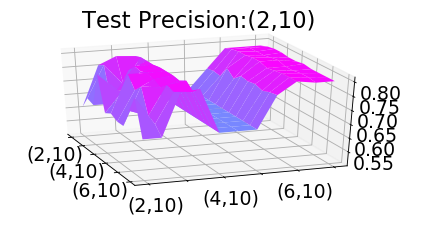
\includegraphics[width=0.32\textwidth]{210}
	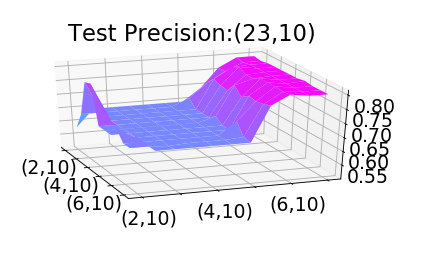
\includegraphics[width=0.32\textwidth]{2310}
	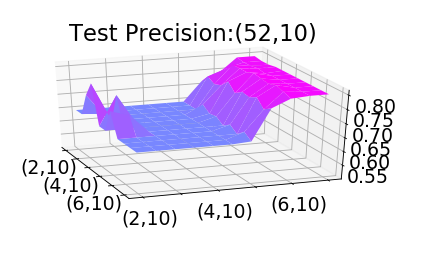
\includegraphics[width=0.32\textwidth]{5210}
\end{figure*}
\section{Background}
The format adopted in floating point representation is the following: the sign of the number, significand (mantissa) and exponent. 
This format is part of the IEEE 754 standard which includes two well known representations: single precision (1-bit sign, 23-bit mantissa, 8-bit exponent) and double precision (1-bit sign, 52-bit mantissa, 11-bit exponent). 
It has been showed \cite{softfloat} the way mantissa and exponent split the total amount of bits in single and double representation can be further improved.

The Perceptron algorithm is a supervised learning algorithm invented by Frank Rosenblatt in 1957\cite{perceptron}. The goal of the predictor is to train a linear decision boundary on a set of labeled samples to classify unknown data in the future.
The Perceptron is a mistake driven algorithm: once a sample is misclassified the predictor is updated but not necessary classified correctly. The update step involves the weight vector, the main actor in the classification process.
Particularly interesting in terms of floating point analysis is the average variant of vanilla Perceptron. 
%The average Perceptron differs from the vanilla version because it maintains an average predictor weighted on the misclassification occurred until the current iteration.%

On the other hand SVM algorithm produces a linear classifier, but it differs from Perceptron in the way the hyperplane is obtained. SVM is much restrictive that Perceptron because it aims for a safe margin between the linear separator and the closest points. We have implemented the soft version of SVM: (i) soft SVM means that points are allowed to exists between the linear separator and the margin. The goal is to maximize the 'safe' margin while minimizing the number of samples violating it.

\section{Methodology}
\subsection{Overview}
Our work consists of re-implementing Perceptron and SVM algorithms using numerical libraries MPFR\cite{MPFR} and \newline FlexFloat\cite{softfloat} such that each floating point instruction can be bounded by a desired floating point format. 
These libraries allow the developer to express how many bit are assigned to mantissa and exponent for their representation.
As a result, our analysis spans lower format configurations allowed for mantissa representation.
In case of exception (only for lack of dynamic range, a lack of precision for mantissa never produces exception) the procedure is stopped, the exponent is increased and the algorithm starts again. 
\subsection{Reading, Training and Testing}
We decide to split the lifetime of the predictor into three different procedures: (i) reading (ii) training (iii) testing. 
The goal of such separation is to detect what are the dependencies between them. We want to stress the combinations of formats used for representations.
 
The first impact of our work is to detect a minimum threshold in the precision to adopt for the dataset representation. Minimizing this precision, while still maintaining high values for the accuracy of predictors ($\frac{Correct.Classification}{Tot.classification}$) results in enormous saving in terms of architecture complexity, energy consumption, computational effort, and memory savage\cite{softfloat}. 
We call this parameter: Precision Dataset.
Once the dataset is masked at the desired FP precision, the training procedure of each algorithm imports it independently. The precision used to compute the training is bounded by precision computing. The interface between reading and computing receives in input the dataset from the parsing procedure and adapt it to the bound fixed by precision computing. 
In the result section, we will see what is the impact of this parameter on a well known binary classification problem.
Finally, the last key point of the analysis is the testing procedure. While performing test on unknown data, the parsing procedure imports the dataset at the same precision used for training.
%\newpage
\section{Results}
Our analysis consists in the implementation of Perceptron (average Variant) and SVM using MPFR\cite{MPFR} library. 
The code is developed using C++ language, and it is publicly available at LINK.
To confirm the results of the analysis the same implementations are replicated using FlexFloat library \cite{softfloat}. We have analyzed the following dataset: fourclass(link), heart(link), diabet(link), .
The analysis is performed on a desktop machine with i7-6700HQ CPU @ 2.60GHz and 16GB RAM. 
These graphs are obtained using matplotlib library. 
DESCRIBE GRAPHS (i) Testing using poor precision results in high accuracy. (ii) dataset precision may not impact on the accuracy: store values in dataset at low precision and save memory space. (iii) conclude about the heterogeneity of datasets. 


%% Acknowledgments
%\begin{acks}                            %% acks environment is optional
%                                        %% contents suppressed with 'anonymous'
%  %% Commands \grantsponsor{<sponsorID>}{<name>}{<url>} and
%  %% \grantnum[<url>]{<sponsorID>}{<number>} should be used to
%  %% acknowledge financial support and will be used by metadata
%  %% extraction tools.
%  This material is based upon work supported by the
%  \grantsponsor{GS100000001}{National Science
%    Foundation}{http://dx.doi.org/10.13039/100000001} under Grant
%  No.~\grantnum{GS100000001}{nnnnnnn} and Grant
%  No.~\grantnum{GS100000001}{mmmmmmm}.  Any opinions, findings, and
%  conclusions or recommendations expressed in this material are those
%  of the author and do not necessarily reflect the views of the
%  National Science Foundation.
%\end{acks}


%% Bibliography
\bibliography{bibfile}


%% Appendix
%\appendix
%\section{Appendix}
%
%Text of appendix \ldots

\end{document}
